\documentclass[landscape,footrule]{foils}
\usepackage[lecture-serie]{foiltex-extra}
\usepackage{crysymb}
\usepackage{graphics}
\usepackage[pdftex]{graphicx} 




\newcommand{\lecture}{Introduction}
\newcommand{\lserie}{LTAT.02.004 Machine Learning II}
\newcommand{\ldate}{10 February, 2020}
\newcommand{\lauthor}{Sven Laur}
\newcommand{\linst}{University of Tartu}
\graphicspath{{./illustrations/}}
\MyLogo{\lserie,\  Introduction to Machine Learning II, \ldate}


\newcommand{\leqm}{\ \leq_m}


\newcommand{\bigvskip}{\vskip 2em}
\newcommand{\lastline}{\vspace*{-2ex}}
\newcommand{\spreadappart}{\vspace*{\fill}}

\DeclareMathOperator{\supp}{supp}
\DeclareMathOperator{\conf}{conf}
\DeclareMathOperator{\precision}{precision}
\DeclareMathOperator{\recall}{recall}


\begin{document}
\titlefoil

\foilhead[-1.5cm]{What is this course about?}
\enlargethispage{1cm}
\illustration[scale=1.1]{course-placement}


\foilhead[-1cm]{Four basic tasks in machine learning}
\enlargethispage{3cm}
\begin{tabbing}
 \hspace*{2cm}\=\hspace*{10cm}\=\kill
   \>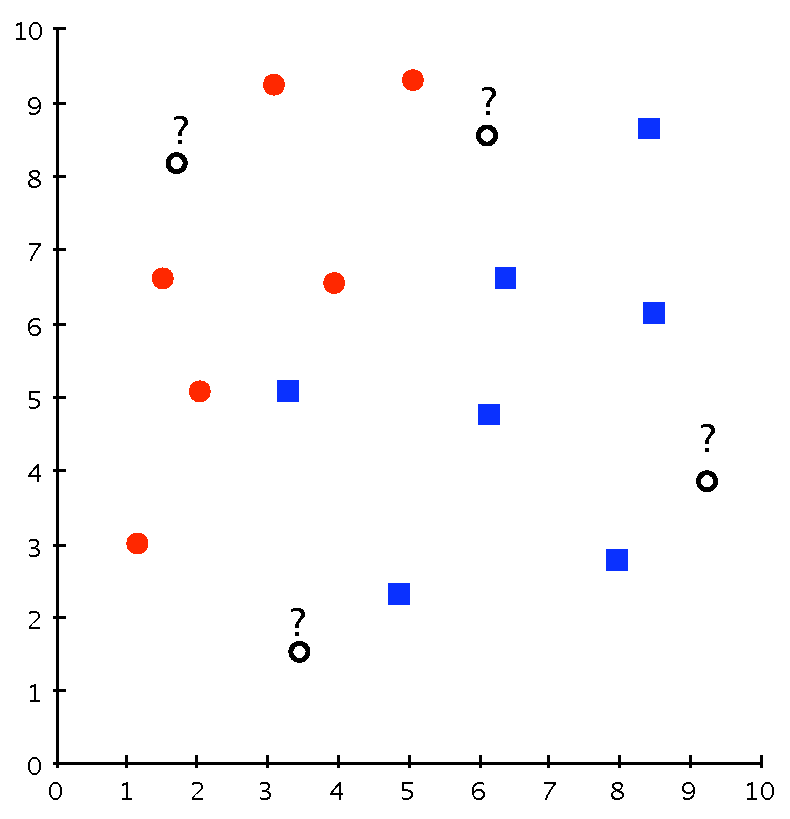
\includegraphics[height = 5.5cm]{classification} \> 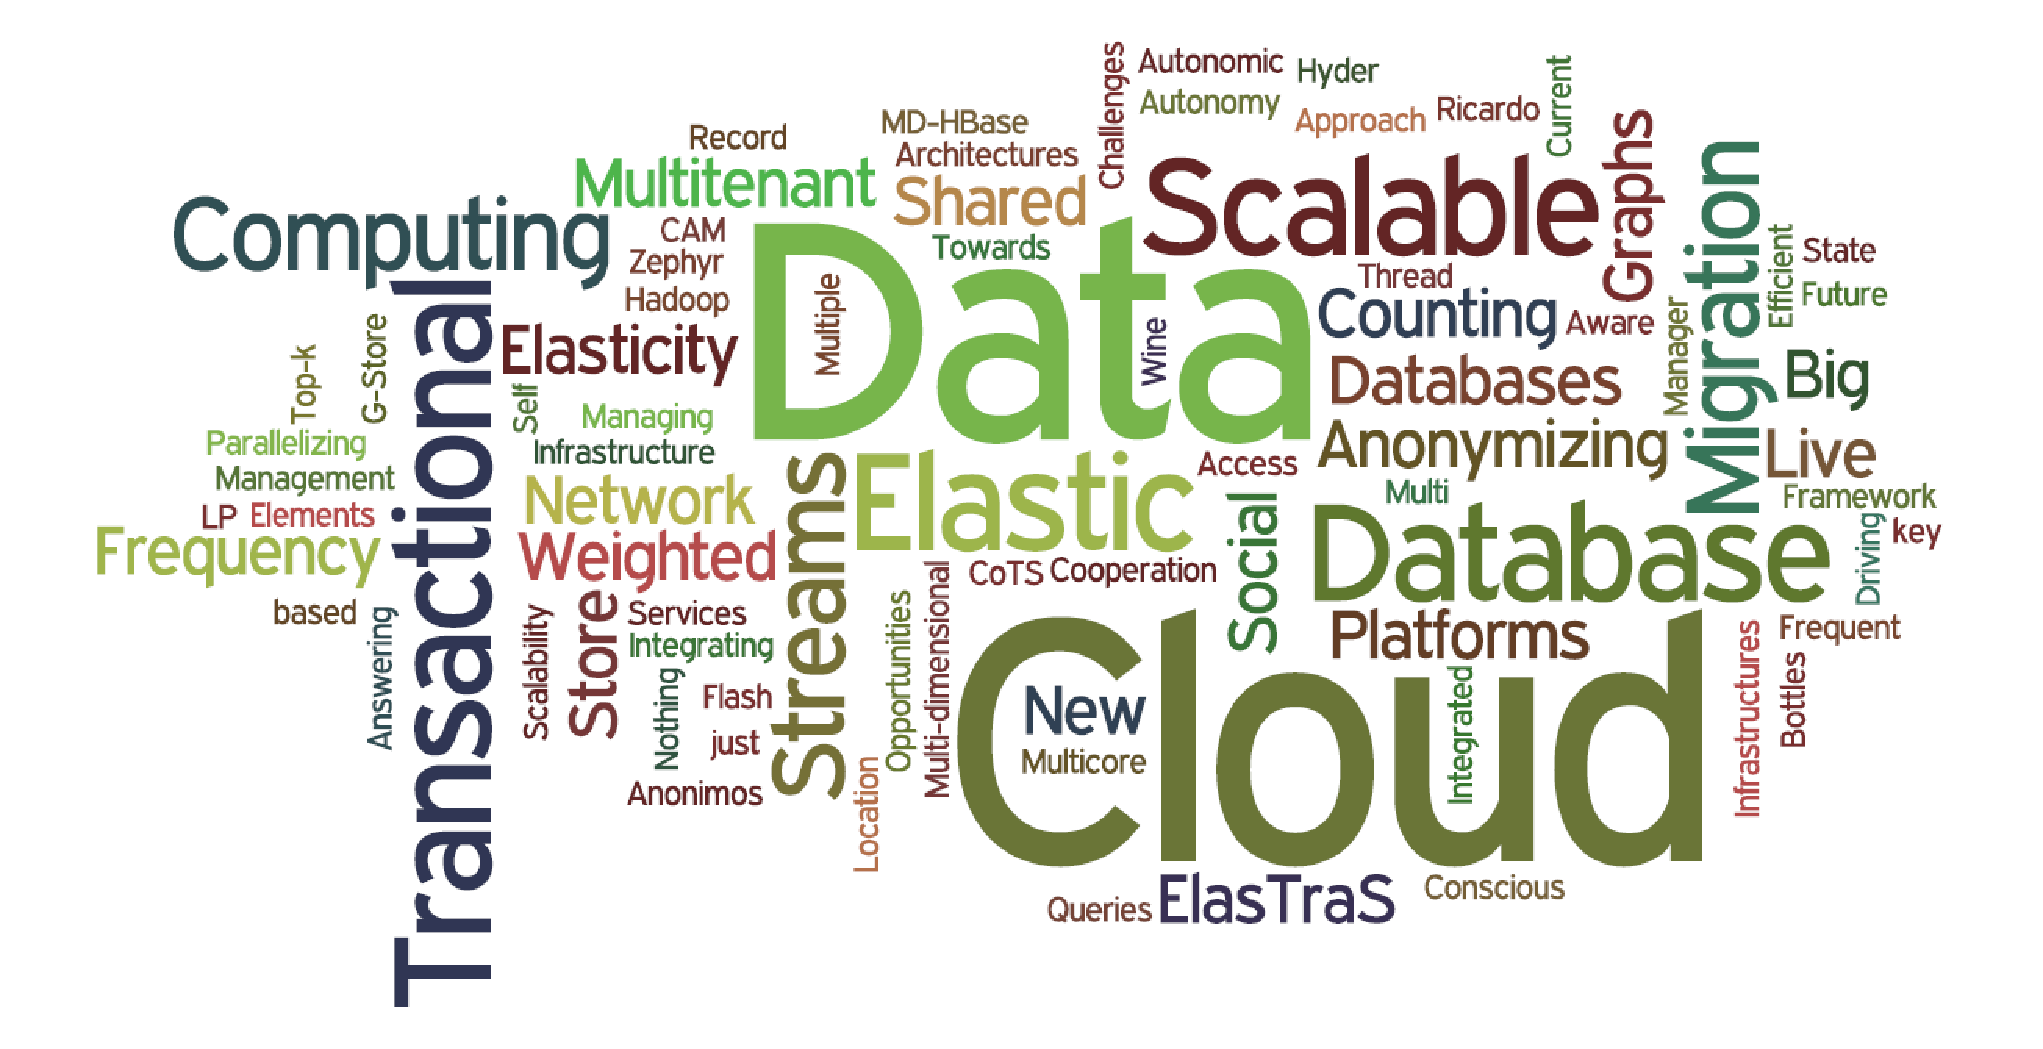
\includegraphics[width = 9cm]{word-cloud}\\  \vspace*{1cm} \\
   \>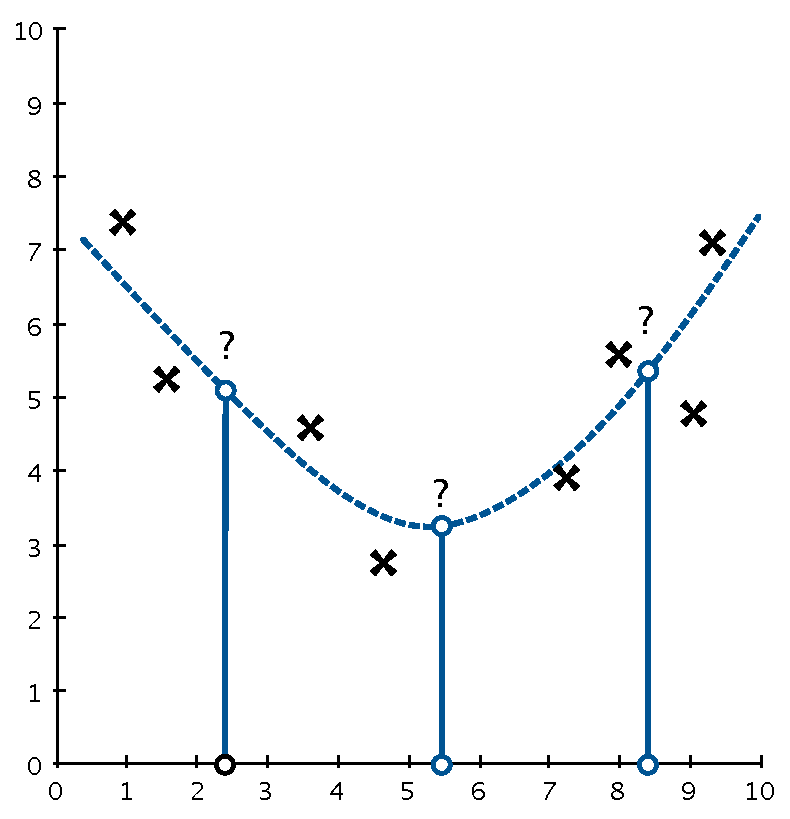
\includegraphics[height = 5.5cm]{regression}   \>  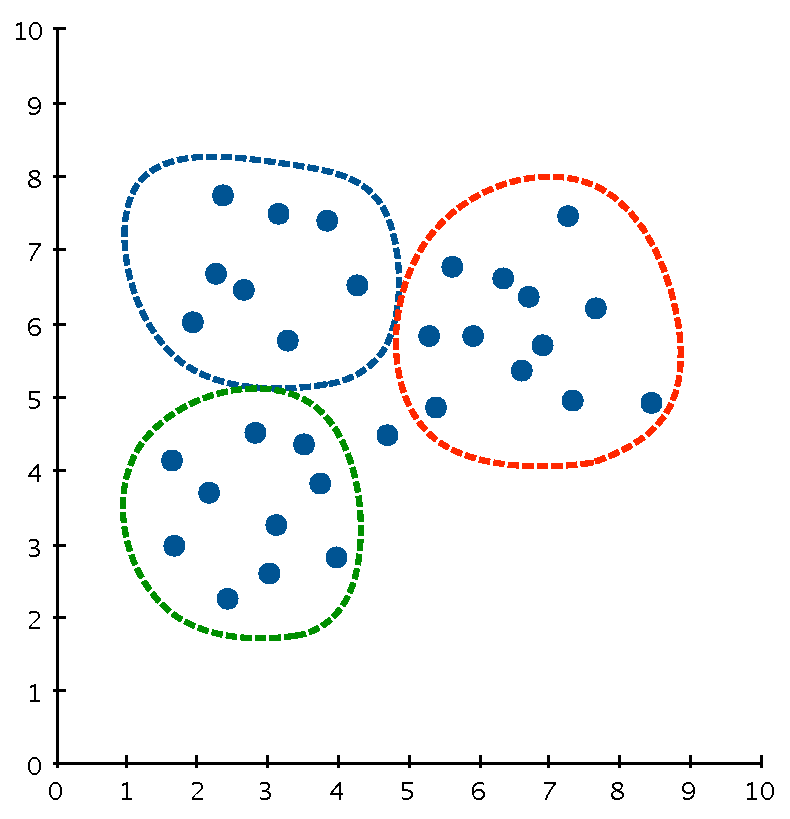
\includegraphics[height =5.5cm]{clustering}\\
\end{tabbing}

\foilhead[-1cm]{Four basic issues you have to solve}

\enlargethispage{3cm}
\begin{tabbing}
 \hspace*{2cm}\=\hspace*{10cm}\=\kill
   \> 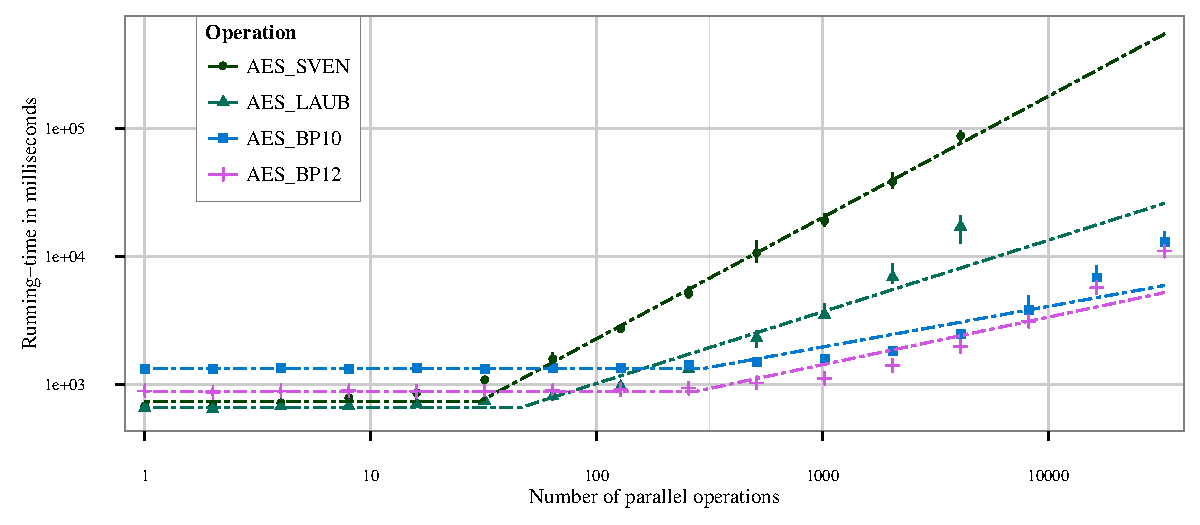
\includegraphics[height = 5.5cm, trim=2.5cm 0cm 3.8cm 0cm, clip]{aes-full-time}
   \> 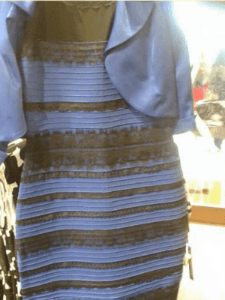
\includegraphics[height = 5.5cm, trim=0cm 0cm 0cm 0cm, clip]{the-dress}
\hspace*{0.15cm}
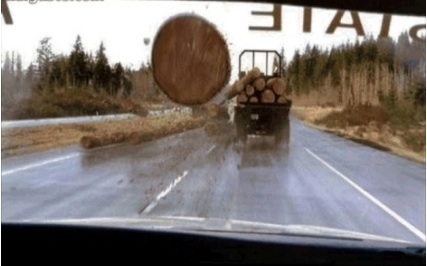
\includegraphics[height = 5.5cm, trim=4cm 0cm 4cm 0cm, clip]{logs-falling}\\

   \> 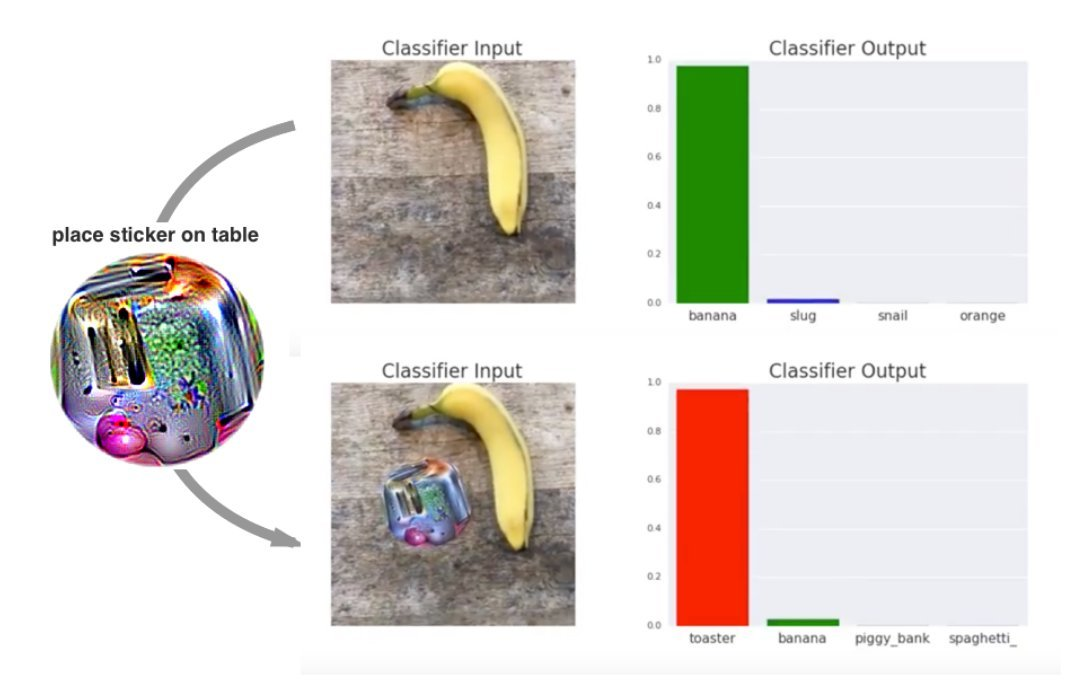
\includegraphics[height = 5.5cm]{adversarial-learning}
   \> 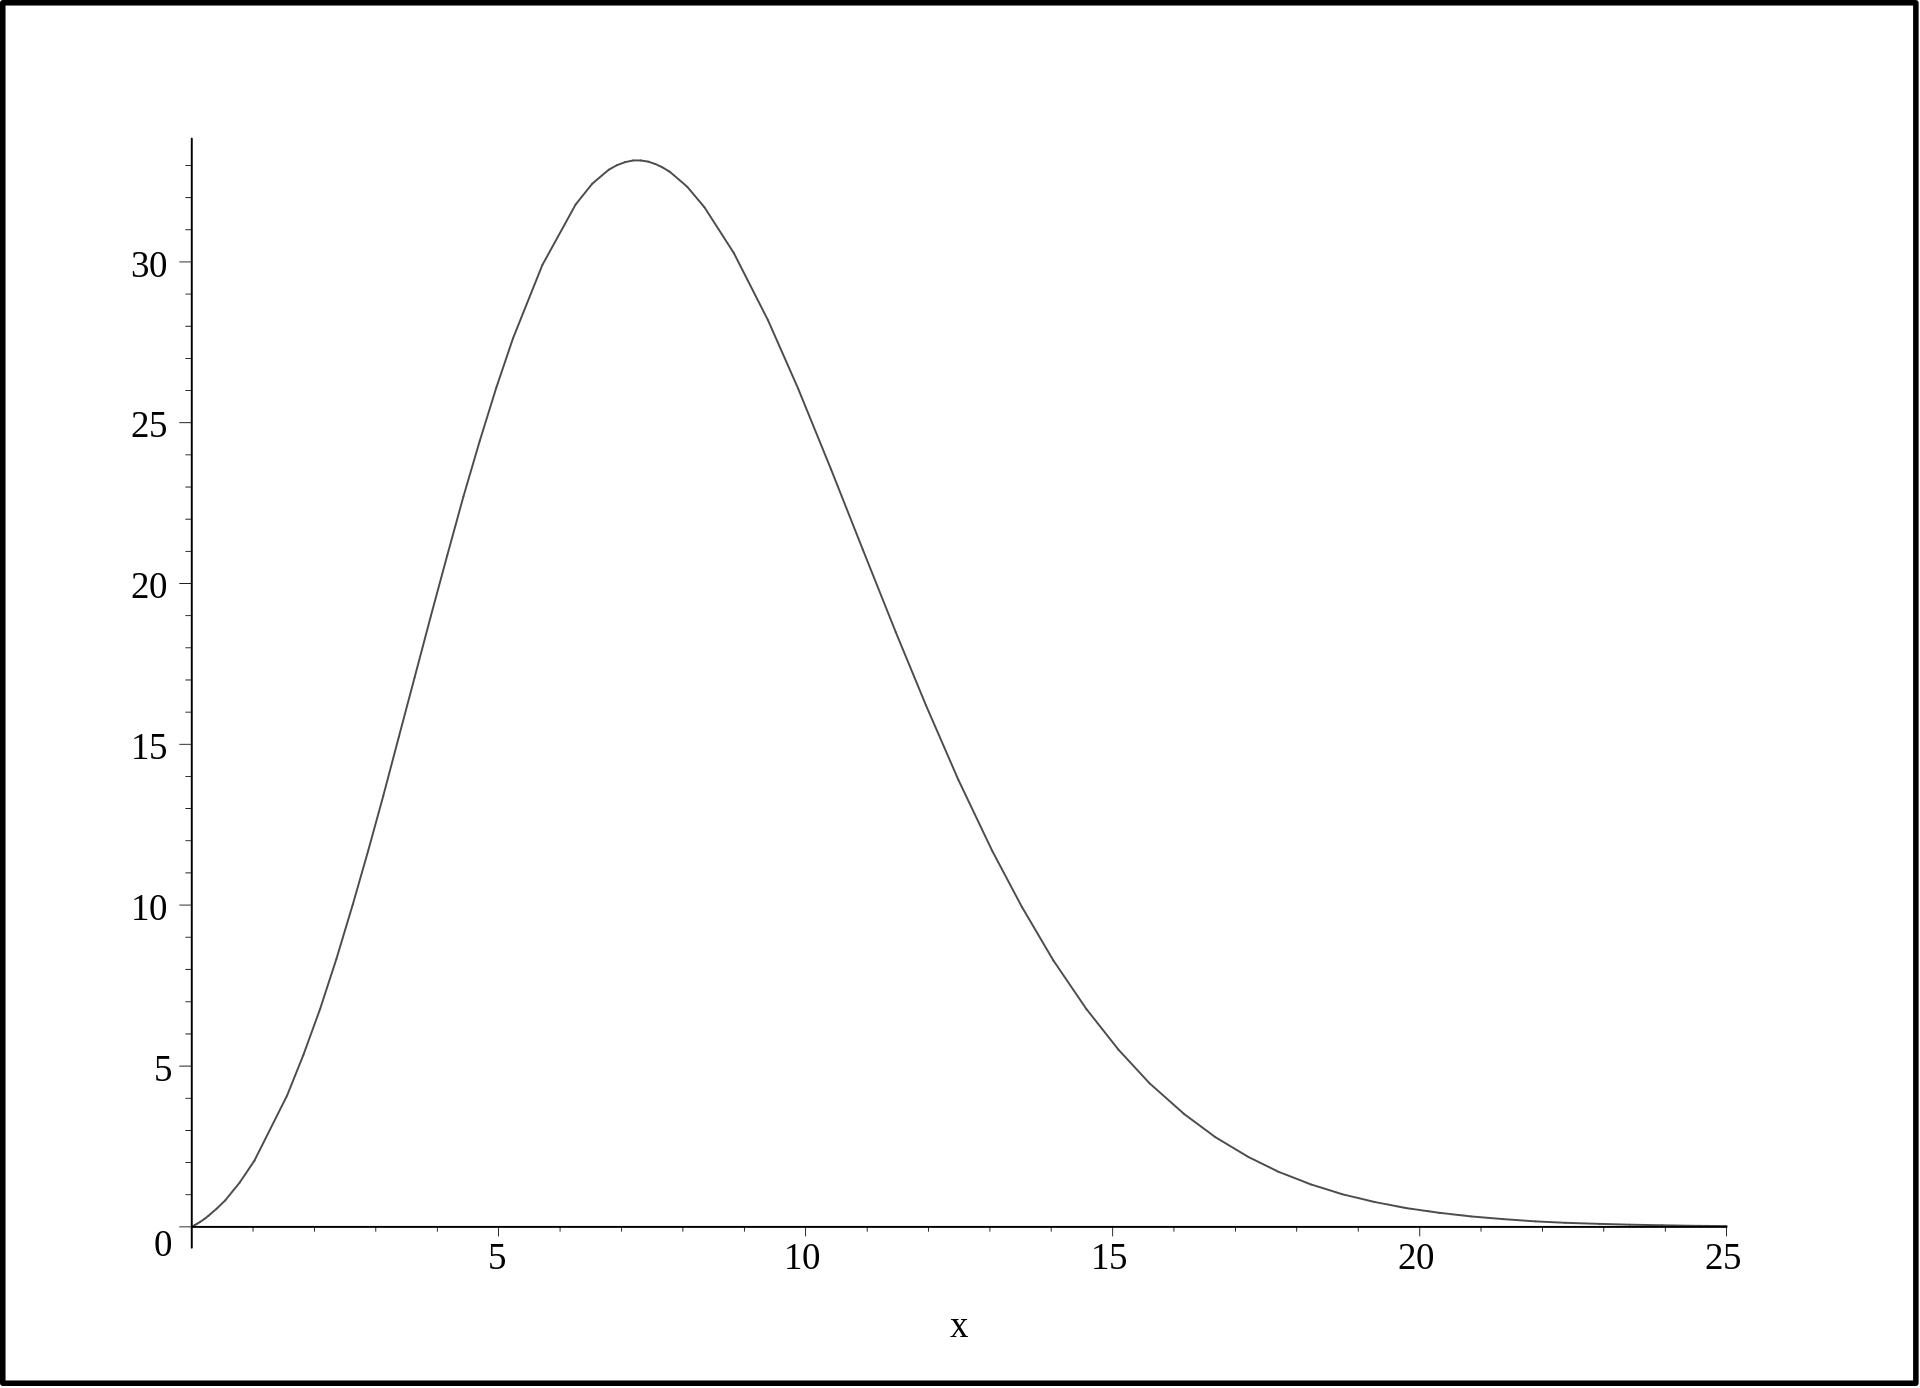
\includegraphics[height = 5.5cm, trim=-4.5cm 0cm -4.5cm 0cm, clip]{curse-of-dimensions}
\end{tabbing}


%\frame{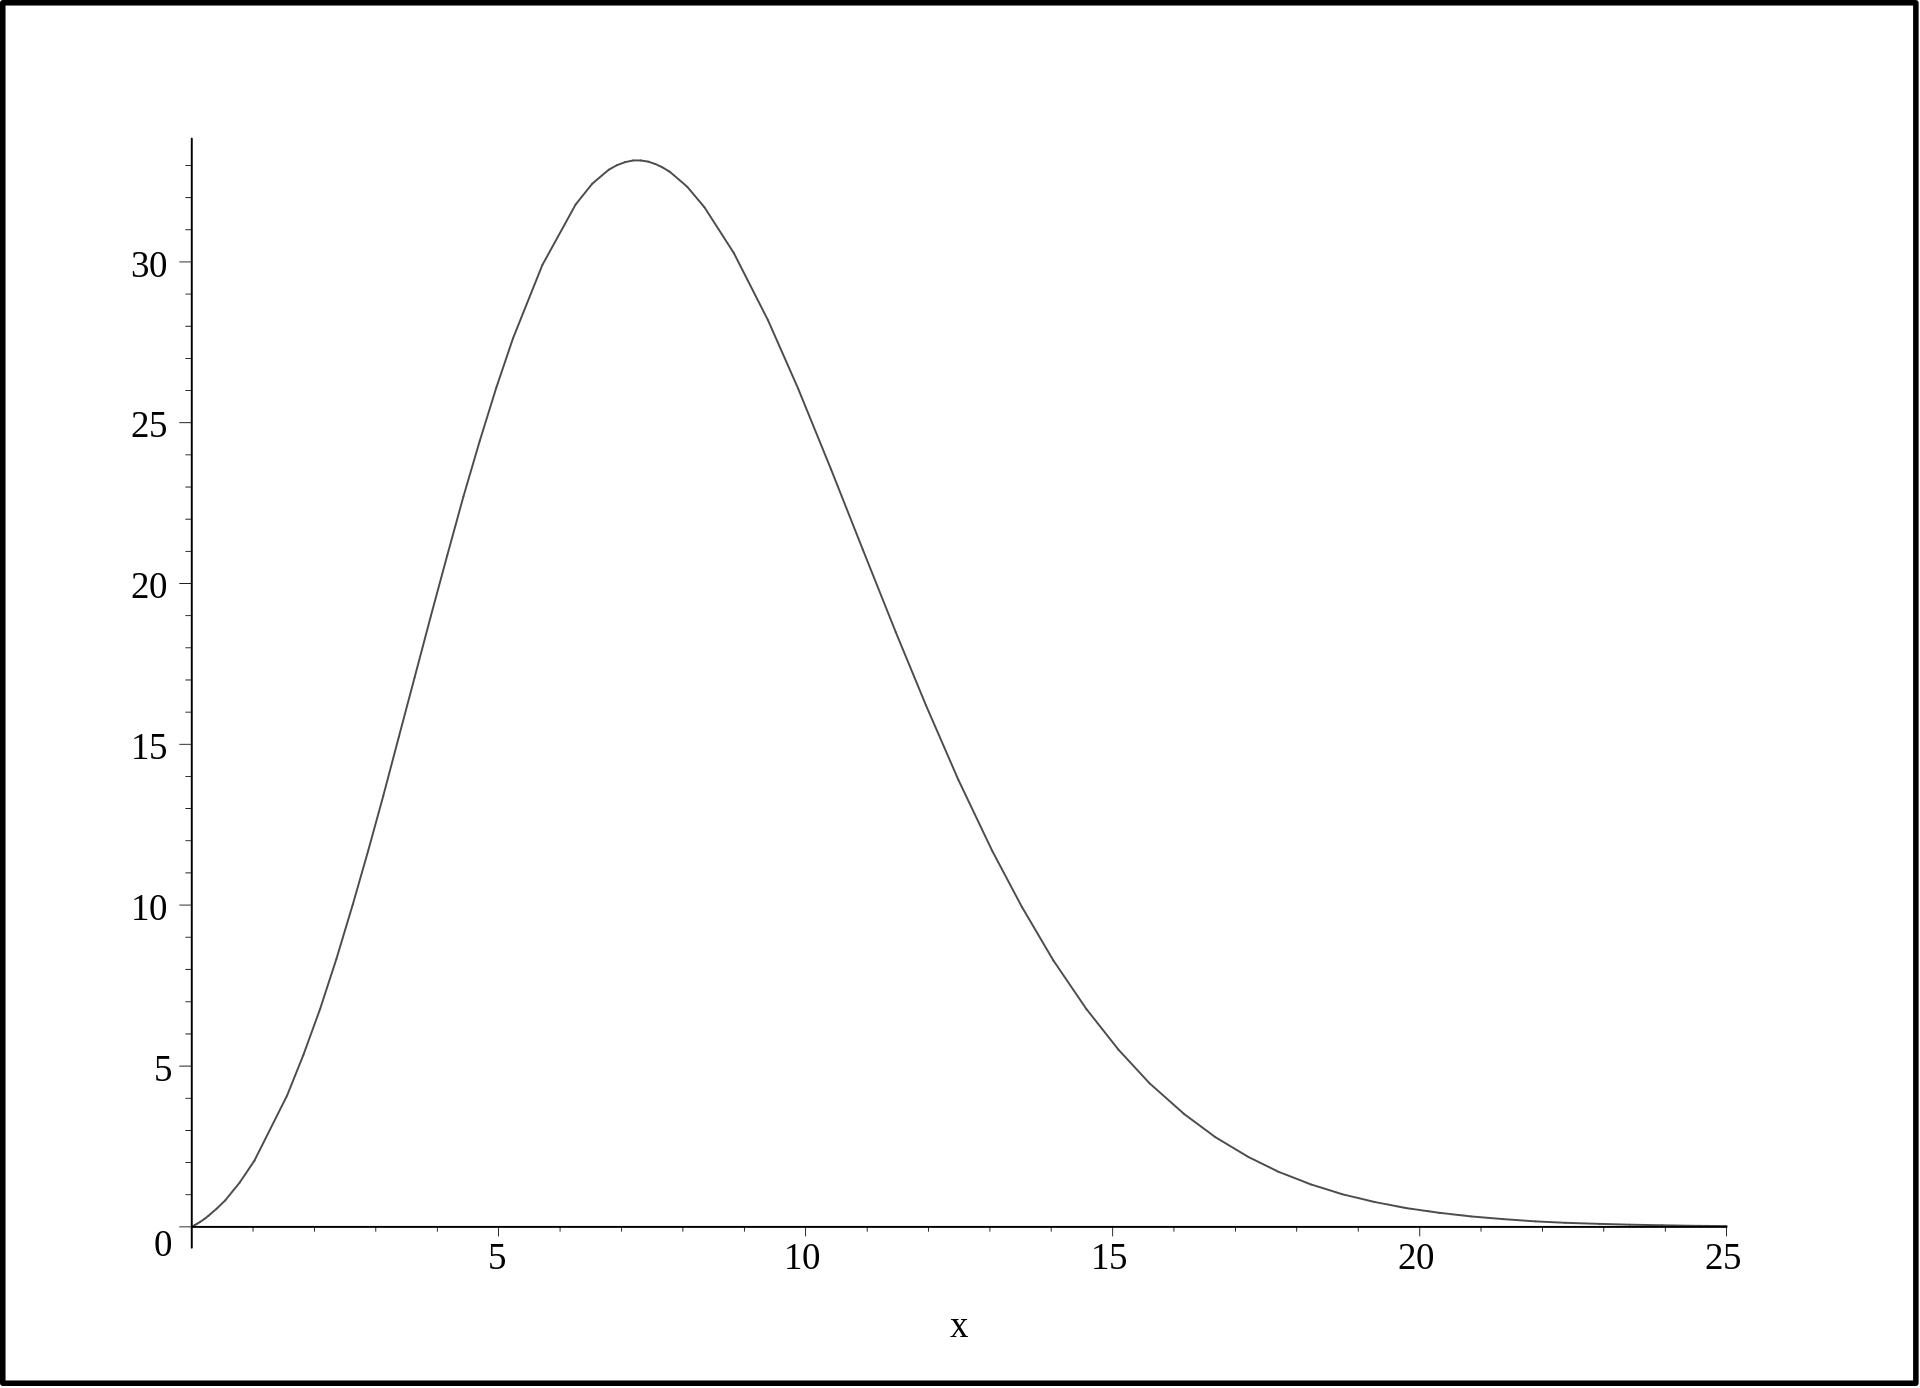
\includegraphics[height = 5.5cm, trim=-4.5cm 0cm -4.5cm 0cm, clip]{curse-of-dimensions}}

\foilhead[-1cm]{Main inference prodedure}

\illustration[height=9cm]{main-procedure}

Usually no machine learning method works on real data without tweaking 
\begin{triangles}
 \item The signal might be missing form the data 
 \item The method uses wrong features for its predictions 
\end{triangles}


\foilhead[-1cm]{Features are more important than method}

\illustration[width=10cm]{checker-board}

The signal is completely lost if we observe a single feature: $x$-coordinate or $y$-coordinate. By knowing both features the pattern is clearly visible.



\foilhead[-1cm]{Do not learn what you already know!}
\illustration[scale=0.8]{physical-modelling}

Sometimes we know the overall structure of the model
\begin{triangles}
 \item In robotics the effect of actuators can be expressed directly
 \item Sometimes we know some governing rules form previous studies
\end{triangles} 
In such cases, learning the entire model with machine learning is wasteful
\begin{triangles}
 \item Locate the parts of the model that are undefined
 \item Use machine learning to find missing links 
\end{triangles} 


\end{document}

